% !TEX root = thesis.tex
%%%%%%%%%%%%%%%%%%%%%%%%%%%%%%%%%%%%%%%%%%%%%%%%%%%%%%%%%%%%%%%%%%%%%%%%%%%%%%%%
\chapter{Анализ подходов и средств инструментирования программ}
%%%%%%%%%%%%%%%%%%%%%%%%%%%%%%%%%%%%%%%%%%%%%%%%%%%%%%%%%%%%%%%%%%%%%%%%%%%%%%%%
%%%%%%%%%%%%%%%%%%%%%%%%%%%%%%%%%%%%%%%%%%%%%%%%%%%%%%%%%%%%%%%%%%%%%%%%%%%%%%%%
\section{Методы повышения качества}
\label{sec:quality_methods}
%%%%%%%%%%%%%%%%%%%%%%%%%%%%%%%%%%%%%%%%%%%%%%%%%%%%%%%%%%%%%%%%%%%%%%%%%%%%%%%%

Существует две группы подходов по обеспечению качества программного
обеспечения~\cite{itsykson}:

\begin{enumerate}
    \item Подходы, основанные на синтезе ПО
    \item Подходы, основанные на анализе уже созданного ПО
\end{enumerate}

Подходы, основанные на синтезе ПО, используют различные формализации во время
проектирования системы, таким образом позволяя избежать ошибок на более поздних
этапах разработки.

Данные формализации включают в себя:

\begin{itemize}
    \item формальные спецификации
    \item формальные и неформальные описания различных аспектов программной
    системы
    \item архитектурные шаблоны и стили
    \item паттерны проектирования
    \item генераторы шаблонов программ
    \item генераторы программ
    \item контрактное программирование
    \item аннотирование программ
    \item верификация моделей программ с использованием частичных спецификаций
    \item использование моделей предметной области для автоматизации
    тестирования программ
\end{itemize}

Подходы, основанные на анализе уже созданного ПО, используется для повышения
качества уже созданного ПО, что позволяет улучшить огромное количество уже
разработанных программных систем, имеющих проблемы с уровнем качества.

%%%%%%%%%%%%%%%%%%%%%%%%%%%%%%%%%%%%%%%%%%%%%%%%%%%%%%%%%%%%%%%%%%%%%%%%%%%%%%%%
\section{Классификация методов обеспечения качества}
%%%%%%%%%%%%%%%%%%%%%%%%%%%%%%%%%%%%%%%%%%%%%%%%%%%%%%%%%%%%%%%%%%%%%%%%%%%%%%%%

Обычно выделяют следующие базовые классификации методов обеспечения
качества~\cite{kulyamin}:

\begin{figure}[h!]
    \begin{center}
        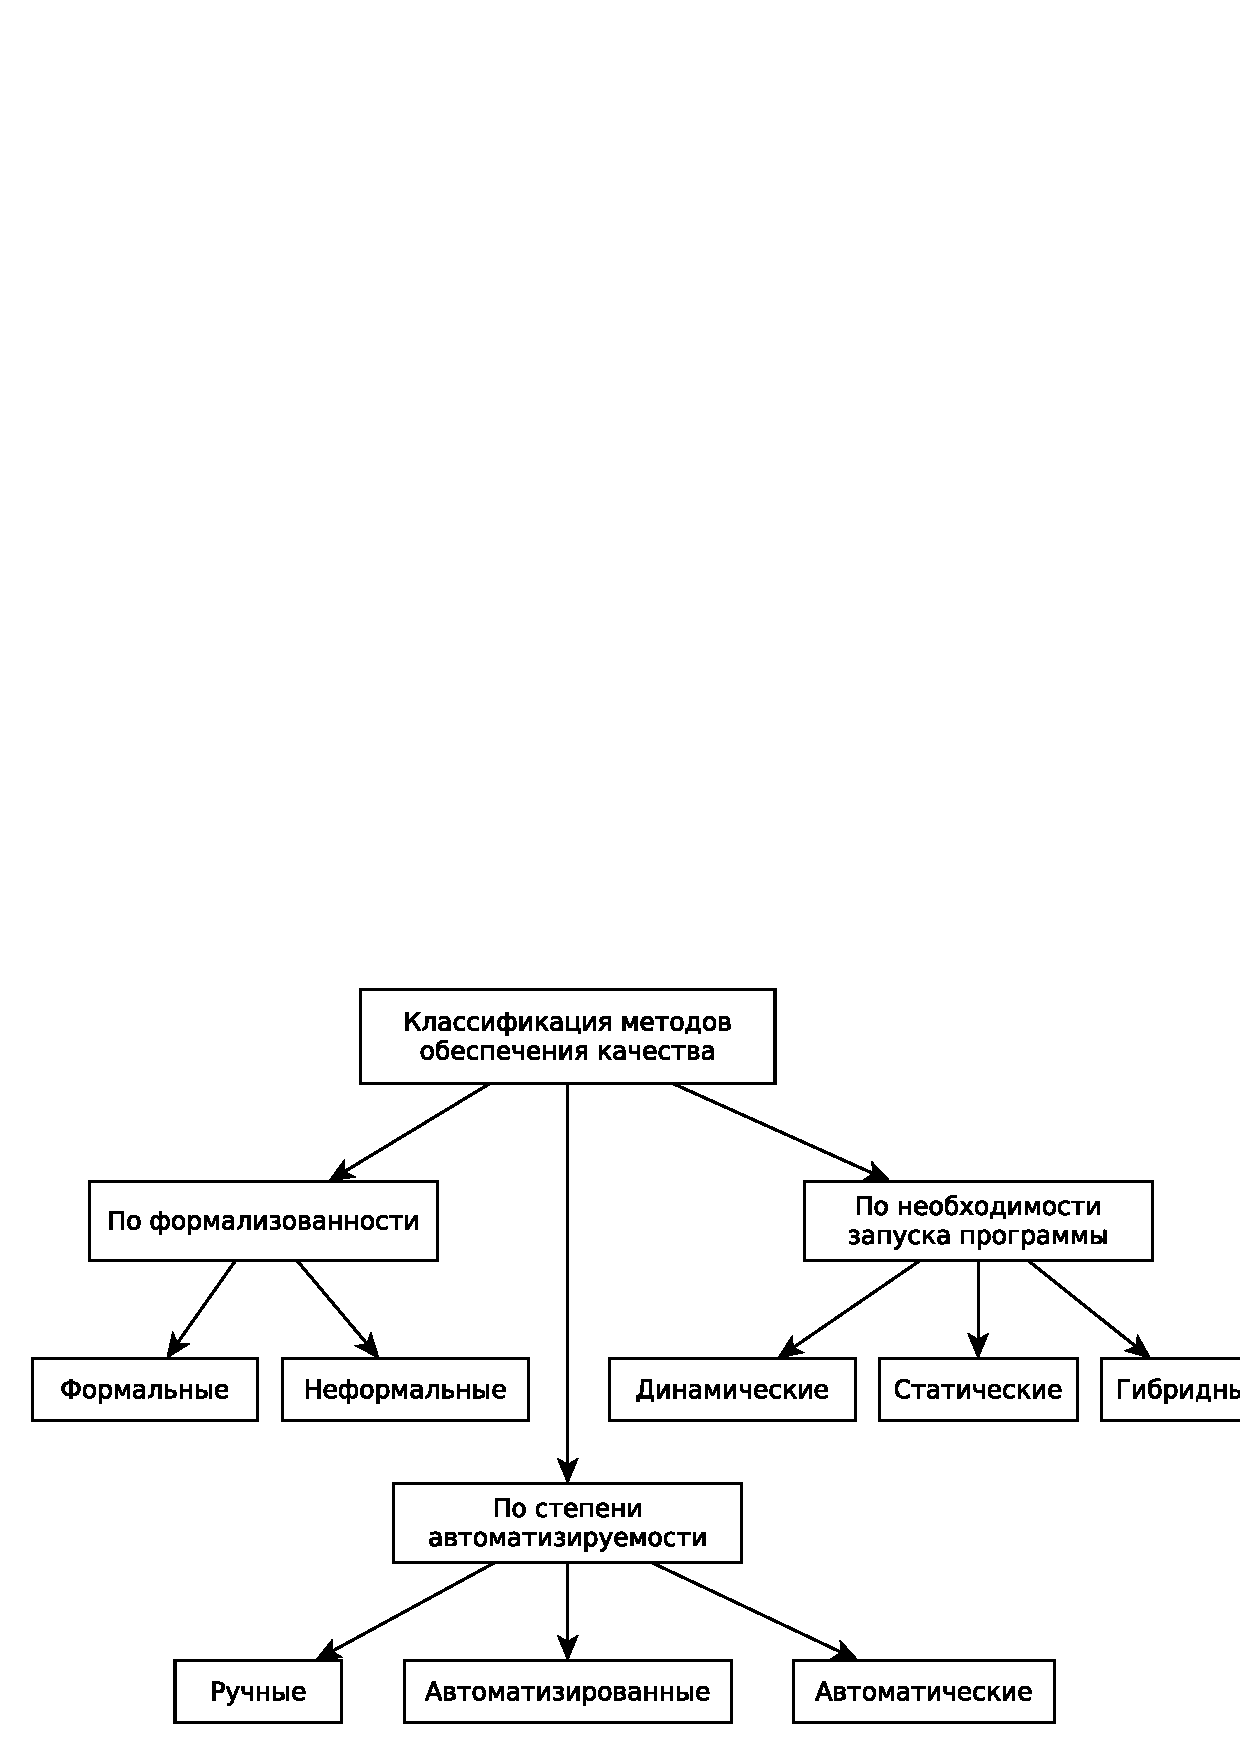
\includegraphics[width=\textwidth]{verification_classification.png}
    \end{center}
    \caption{Схема используемой классификации методов верификации}
    \label{fig:verification_classification}
\end{figure}

\textbf{Экспертиза} позволяет находить ошибки, используя различные артефакты
жизненного цикла системы, в отличие от формальных и динамических методов, и
позволяет находить большое множество разновидностей ошибок. К ее недостаткам
можно отнести невозможность автоматизации.

\textbf{Статический анализ} - это процесс выявления ошибок и недочетов в
исходном коде программ. От остальных методов верификации его отделяет то, что
статический анализ использует только исходные тексты программы, что позволяет
обнаруживать ошибки на стадии написания кода. Таким образом, при анализе
отсутствует спецификация программы - описание того, что она делает. Это
уменьшает множество обнаруживаемых ошибок, но позволяет полностью
автоматизировать процесс анализа.

\textbf{Формальные методы} позволяют создавать формальные функциональные
спецификации и модели архитектуры систем, а также осуществлять их преобразование
в программы с последующей верификацией~\cite{formal_methods}. Корректность
полученных результатов гарантируется математическим аппаратом. К таким методам
относятся, например, дедуктивная верификация, проверка моделей и абстрактная
интерпретация.

Эти методы можно применить только к тем свойствам, которые можно выразить в
рамках некоторой математической модели. Построение этой модели не
автоматизируется, а провести анализ таких моделей может лишь специалист. Однако
сама проверка свойств может быть автоматизирована и позволяет находить даже
самые сложные ошибки.

\textbf{Динамические методы} используются для анализа и оценки свойств
программной системы по результатам ее реальной работы. Одними из таких методов
являются тестирование и анализ трасс исполнения.

Для применения данных методов необходимо иметь работающую систему (или ее
прототип), поэтому их нельзя использовать на ранних стадиях разработки. Также
данные методы позволяют найти только те ошибки в ПО, которые проявляются в его
работе.

\textbf{Синтетические методы} объединяют в себе элементы некоторых способов
повышения качества, описанных выше. Например, существуют динамические методы,
использующие элементы формальных - тестирование на основе моделей (model driven
testing)~\cite{Vieira2006} и мониторинг формальных свойств (runtime
verification)~\cite{runtime_verification}. Цель таких методов - объединить
преимущества уже используемых подходов.

%%%%%%%%%%%%%%%%%%%%%%%%%%%%%%%%%%%%%%%%%%%%%%%%%%%%%%%%%%%%%%%%%%%%%%%%%%%%%%%%
\section{Модели программных систем}
\label{sec:system_models}
%%%%%%%%%%%%%%%%%%%%%%%%%%%%%%%%%%%%%%%%%%%%%%%%%%%%%%%%%%%%%%%%%%%%%%%%%%%%%%%%

Одной из важнейших составляющих анализа программных систем является построение
модели. Без нее анализатор будет вынужден непосредственно оперировать с исходным
кодом, что влечет за собой усложнение процедур анализа и самого анализатора в
целом.

В зависимости от способа построения и назначения модели, они могу различаться по
структуре и сложности и обладать различными свойствами. Существуют следующие
виды моделей~\cite{itsykson}:

\begin{itemize}
    \item Структурные модели
    \item Поведенческие модели
    \item Гибридные модели
\end{itemize}

Структурные модели во основном используют информацию о синтаксической структуре
анализируемой программы, в то время как поведенческие - информацию о
динамической семантике. Гибридные модели используют оба этих подхода.

\subsubsection{Структурные модели}
\begin{enumerate}
    \item Синтаксическое дерево

    Синтаксическое дерево является результатом разбора программы в
    соответствии с формальной грамматикой языка программирования. Вершины
    этого дерева соответствуют нетерминальным символам грамматики, а листья
    - терминальным.

    \item Абстрактное синтаксическое дерево

    Данная модель получается из обычного синтаксического дерева путем
    удаления нетерминальных вершин с одним потомком и замены части
    терминальных вершин их семантическими атрибутами.
\end{enumerate}

\subsubsection{Поведенческие модели}
\begin{enumerate}
    \item Граф потока управления

    Граф потока управления представляет потоки управления программы в виде
    ориентированного графа. Вершинами графа являются операторы программы, а дуги
    отображают возможный ход исполнения программы и связывают между собой
    операторы, выполняемые друг за другом.

    \item Граф зависимостей по данным

    Граф зависимостей по данным отображает связь между конструкциями программы,
    зависимыми по используемым данным. Дуги графа соединяют узлы, формирующие
    данные, и узлы, использующие эти данные.

    \item Граф программных зависимостей

    Данная модель объединяет в себе особенности графа потока управления и графа
    зависимости по данным. В графе программных зависимостей присутствуют дуги
    двух типов: информационные дуги отображают зависимости по данным, а
    дуги управления соединяют последовательно выполняемые конструкции.

    \item Представление в виде SSA

    Однократное статическое присваивание (static single assignment) -
    промежуточное представление программы, которое обладает следующими
    свойствами:
        \begin{itemize}
            \item Всем переменным значение может присваиваться только один раз.
            \item Вводится специальный оператор $\phi$-функция, который
            объединяет разные версии локальных переменных.
            \item Все операторы программы представляются в трехоперандной форме.
        \end{itemize}
\end{enumerate}

\subsubsection{Гибридные модели}
\begin{enumerate}
    \item Абстрактный семантический граф

    Данная модель является расширением абстрактного синтаксического дерева путем
    добавления дуг, отражающих некоторые семантически свойства программы,
    например, такие дуги могут связывать определение и использование переменной
    или определение функции и ее вызов.
\end{enumerate}

%%%%%%%%%%%%%%%%%%%%%%%%%%%%%%%%%%%%%%%%%%%%%%%%%%%%%%%%%%%%%%%%%%%%%%%%%%%%%%%%
\section{Постановка требований к инструментальной среде}
%%%%%%%%%%%%%%%%%%%%%%%%%%%%%%%%%%%%%%%%%%%%%%%%%%%%%%%%%%%%%%%%%%%%%%%%%%%%%%%%
%%%%%%%%%%%%%%%%%%%%%%%%%%%%%%%%%%%%%%%%%%%%%%%%%%%%%%%%%%%%%%%%%%%%%%%%%%%%%%%%
\section{Анализ существующих решений}
%%%%%%%%%%%%%%%%%%%%%%%%%%%%%%%%%%%%%%%%%%%%%%%%%%%%%%%%%%%%%%%%%%%%%%%%%%%%%%%%
